\section{Overview}


The elements composing the detector, listed in Section~\ref{intro:detector}, include the time projection chamber (TPC), the cold electronics (CE), and the photon detection system (PDS).  The TPC components, e.g., anode planes, a cathode plane and a field cage, are designed in a modular way.  
The six APAs are arranged into two APA planes, each consisting of three side-by-side APAs. Between them,  
a central cathode plane, composed of 18 CPA modules, splits the TPC volume into two electron-drift regions, one on each side of the cathode plane. 
A field cage (FC) completely surrounds the four
open sides of the two drift regions to ensure that the electric field within is uniform and unaffected by the presence of the cryostat walls and other nearby conductive structures. The sections in this chapter describe the components individually.


Figure~\ref{fig:protodune-sp-tpc-touramanis} illustrates how these components fit together. The FC is shown in Figure~\ref{fig:fc-overview}.


Table~\ref{tab:tpc-components} lists the principal detection elements of ProtoDUNE-SP along with their approximate dimensions and their quantities. 

\begin{cdrtable}[TPC detection components, dimensions and quantities]{lll}{tpc-components}{TPC detection components, dimensions and quantities}
Detection Element & Approx Dimensions  & Quantity   \\  \toprowrule
APA          & 6~m H by 2.4~m W  & 3 per anode plane, 6 total  \\  \colhline
CPA module  & 2~m H by 1.2~m W  & 3 per CPA column,   \\  
  &  & 18 total in cathode plane    \\  \colhline
 Top FC module & 2.4~m W by 3.6~m along drift & 3 per top FC assembly, 6 total   \\  \colhline
 Bottom FC module & 2.4~m W by 3.6~m along drift & 3 per bottom FC assembly, 6 total   \\  \colhline
End-wall FC module & 1.5~m H by 3.6~m along drift & 4 per end-wall assembly (vertical   \\  
&  & drift volume edge), 16 total   \\  \colhline
PD module  & 2.2 m $\times$ 86 mm $\times$ 6 mm & 10 per APA, 60 total  \\ 
\end{cdrtable}


\begin{cdrfigure}[The field cages]{fc-overview}{A view of the TPC field cage and the central cathode plane (CPA). The APA that would be positioned at the open end of the FC, and thus obscure the CPA, is not shown.}
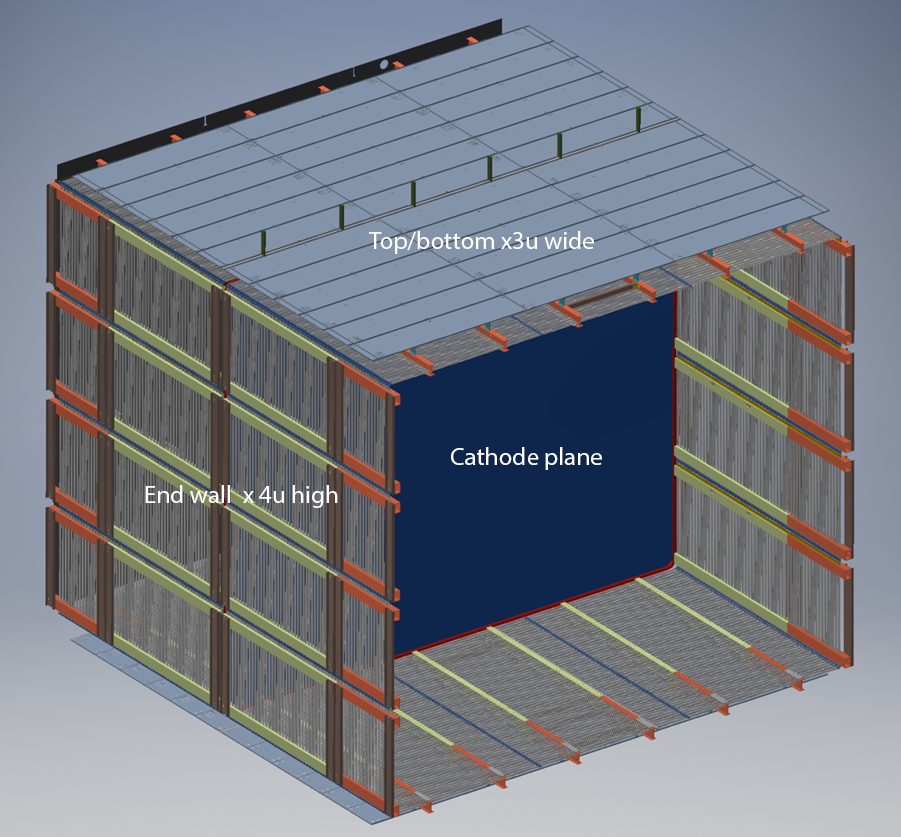
\includegraphics[width=0.6\linewidth]{tpc_fc_overview.png}
\end{cdrfigure}
